\chapter{Software}
\section{The software architecture}
The architecture of program is followed 3-tier model. There-tier architecture is an architecture that each tier is designed, developed and maintained as independent. The advantage of this architecture is intended to allow any upgraded or replaced independent between the tiers. When user want to change the requirements or technology of a tier, it will non-affect to other tiers.\\[0.3cm]
The architecture of three-tiers includes:
\begin{itemize}
	\item \textbf{Data tier}: includes the classes which were designed for the data structure of program. It also provides the persistence mechanism to access the data.
	\item \textbf{Logic tier}: controls the functionality of application by performing detailed processing.
	\item \textbf{Presentation tier}: displays information related to user. It is a layer which received the require from user to program or return the result from program to user. 
\end{itemize}
\begin{figure}[h]
	\centering
	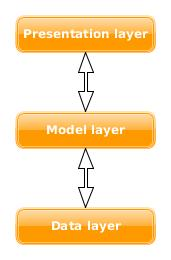
\includegraphics[scale=0.7]{images/software_3tiers}
	\caption{Three-tiers model}
	\label{fign3iters}
\end{figure}
\section{The modules}
The MAELab software mainly includes four modules: \textbf{segmentation}, \textbf{histograms}, \textbf{pht} and \textbf{correlation}. Besides, the software also includes the other modules to support for the main modules. The relation between the modules in the software is shown in figure \ref{fignsmodules}.
\begin{figure}[h]
	\centering
	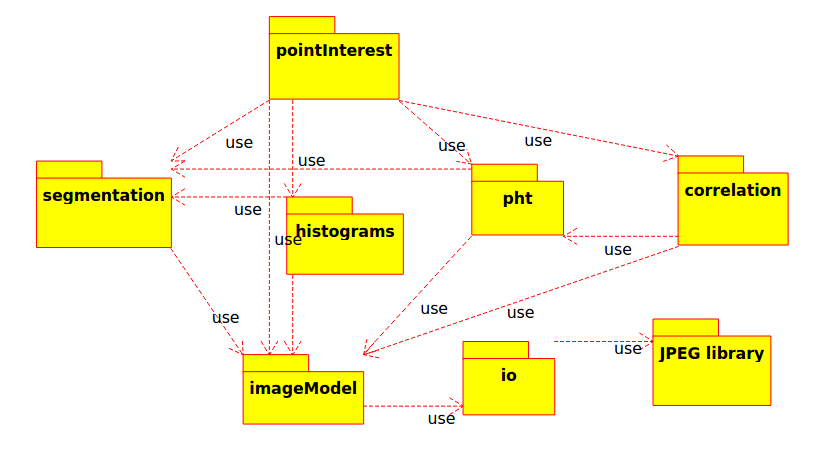
\includegraphics[scale=0.5]{images/modules}
	\caption{Three-tiers model}
	\label{fignsmodules}
\end{figure}
The functions of each modules is describing as followed:
\begin{itemize}
	\item \textbf{io} module: Implement the functions to read and write file. It includes the \textbf{JPEG library} that used to decode and encode the JPEG image.
	\item \textbf{imageModel} module: Represent the data structure of the image.
	\item \textbf{segmentation} module: Implement the segmentation methods on image.
	\item \textbf{histograms} module: Contains the methods to compute the geometric histogram of the image.
	\item \textbf{pht} module: Describe the probabilistic hough transform duration.
	\item \textbf{correlation} module: Includes the template matching methods.
	\item \textbf{pointInterest} module: Combine the result of the modules such as segementation, histograms,... to provide the adapter to other module or other software.
\end{itemize}
\section{The classes architecture}
Figure \ref{figclassdiagram} describes the classes diagram of the software. Based on structurally software, the classes is divided into two parts: one, describing for the data structure and another, describing the functions of software.
\begin{figure}[!h]
	\centering
	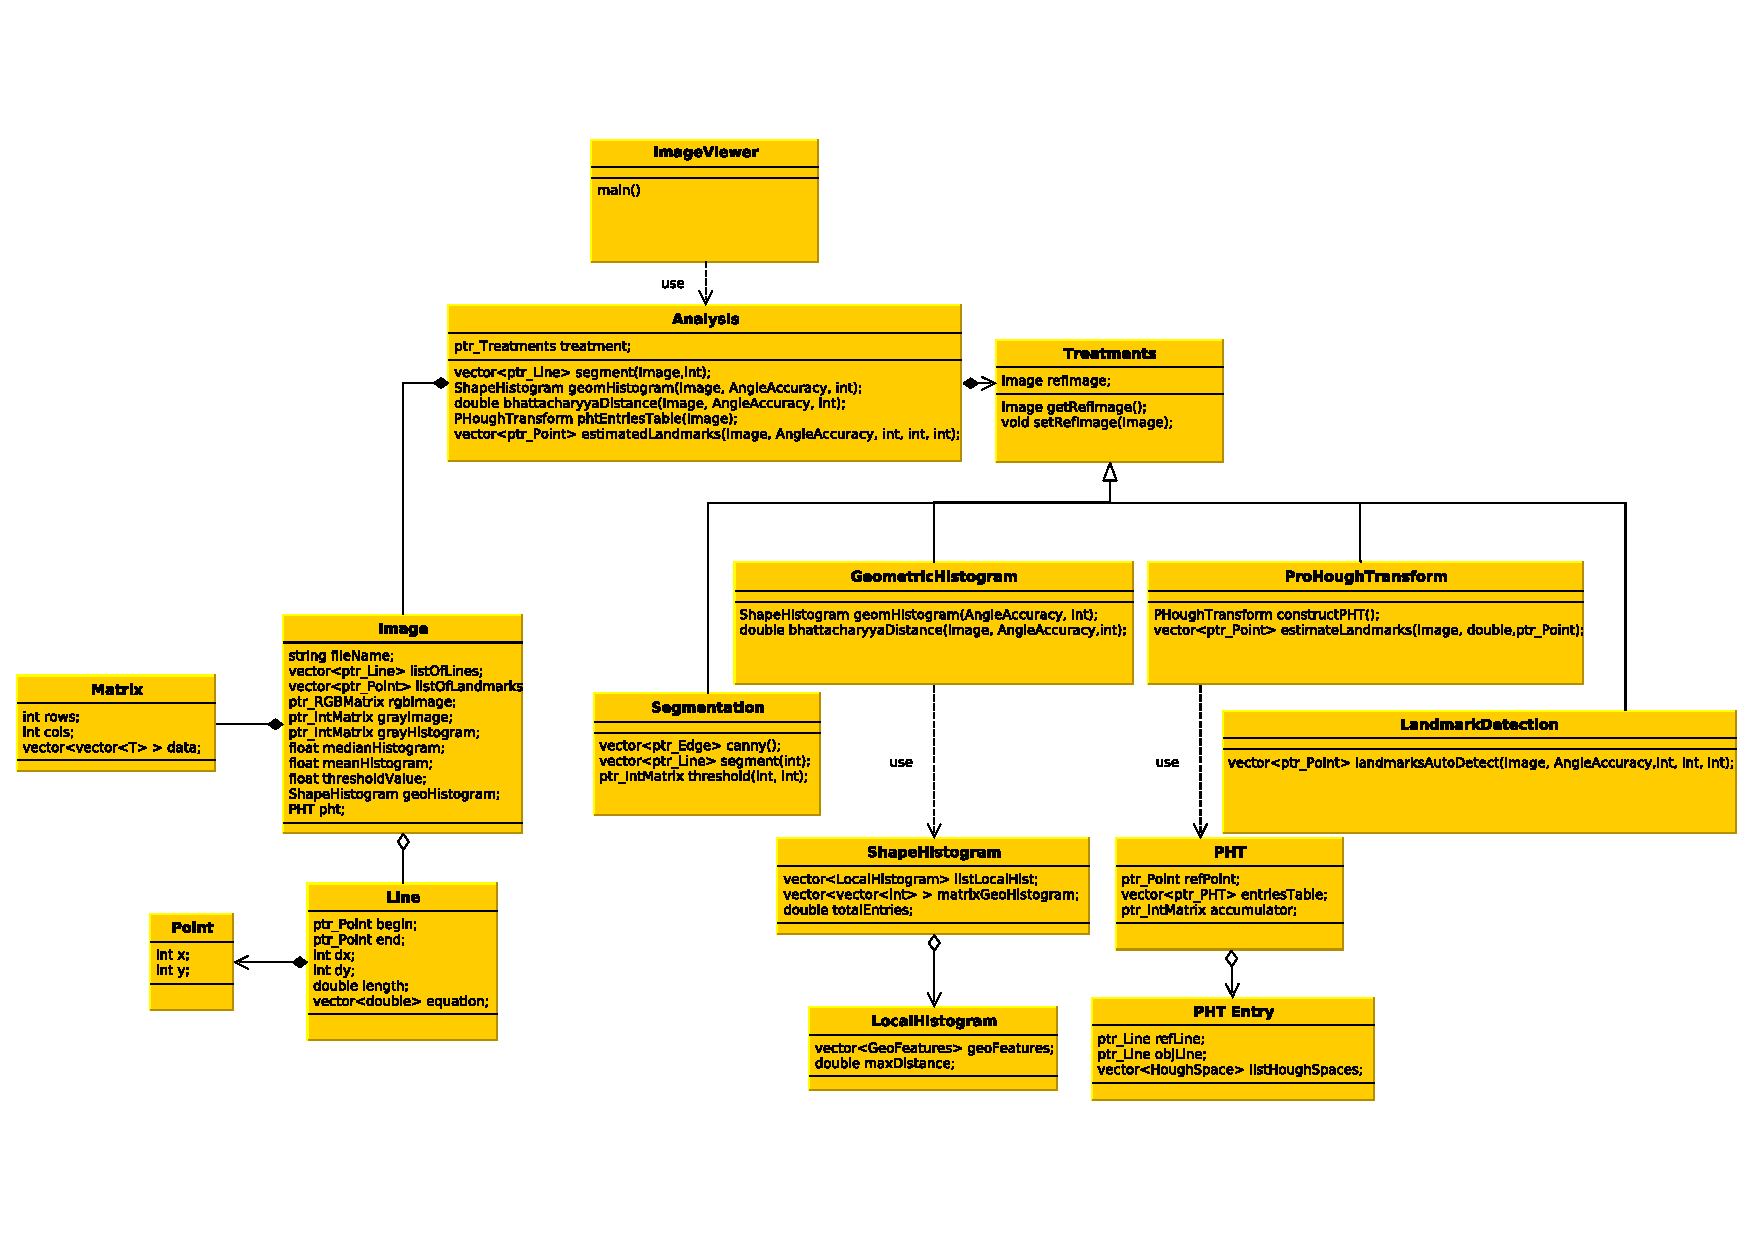
\includegraphics[scale=0.8, angle = -90]{images/classDiagram}
	\caption{Classes diagram}
	\label{figclassdiagram}
\end{figure}
\subsection{Data structure classes}
The data structure classes are the classes that used to represent the structure of the image in program. These classes are using through all the functions of the software.
\begin{itemize}
	\item \texttt{Point} class describes a point in mathematics, its attributes include the coordinate of the point in Cartesian coordinate system.
	\item \texttt{Line} class describes for a straight line. It includes two endpoints and the line's methods, such as: \textit{length of line, perpendicular distance, angle between two lines}. \textit{Line} has been used in more functions of software.
	\item \texttt{Edge} class is an intermediary class. It stores the information of the image at the beginning; after that, its information is used to construct the approximated lines of the image.
	\item \texttt{Matrix} class is used to store the information of the image after decoding.
	\item \texttt{Image} class presents the information of an image (i.e file name, list of edges, matrix that represent the image). It also provides the methods on image such as computing histogram of image, converting image, reading the manual landmarks.
\end{itemize} 
\subsection{Function classes}
The function classes are contains the methods to implement the processes on the image. They are separated into four groups: segment the image, calculate the pairwise geometric histogram of the image, apply the probabilistic hough transform on image and estimate the landmarks on image.
\begin{itemize}
	\item \texttt{Segmentation} classes implement the method to apply the segmentation methods on image such as threshold method, Canny algorithm. It also includes the methods to extract the edge of the image or change the display form of the image into approximated lines.
	\item \texttt{Pairwise geometric histogram} classes provide the method to compute the geometric histogram of the image and measure the difference metric between two images.
	\item \texttt{Probabilistic Hough Transform} classes are implemented to detect the presence of the scene image in the model image. At the beginning, the classes detect the reference point of the model in the scene, and the last result of this process is estimating the manual landmarks of model image in the scene image.
	\item \texttt{Estimating the landmarks} classes provides the methods to verify the estimated landmarks that are detected by probabilistic hough transform. These classes have also methods to evaluate the correctness of the estimated landmarks position.
\end{itemize}